\section{Machines}
During the game Calcifer can use some debris to temporarily transform his lantern in some useful machines.

In the game there are many piles of debris, but in order to build a machine Calcifer needs the proper components.

In order to unlock a new machine, the player has to solve a puzzle. Once unlocked, a machine can be used anytime the player finds a pile of debris with the proper components.

\begin{longtable}[H]{|p{1.7cm}|p{1.7cm}|p{1.7cm}|p{1.7cm}|p{1.7cm}|p{1.7cm}|p{1.7cm}|p{1.7cm}|}
  \hline
\cellcolor[HTML]{656565}{\color[HTML]{FFFFFF} \textbf{Machine}} & \cellcolor[HTML]{C0C0C0}{\color[HTML]{330001} \textbf{First steps}} & \cellcolor[HTML]{C0C0C0}{\color[HTML]{330001} \textbf{Where is Howl?}} & \cellcolor[HTML]{C0C0C0}{\color[HTML]{330001} \textbf{In enemy territory}} & \cellcolor[HTML]{C0C0C0}{\color[HTML]{330001} \textbf{Nasty surprise(s)}} & \cellcolor[HTML]{C0C0C0}{\color[HTML]{330001} \textbf{The djiin of the desert}} & \cellcolor[HTML]{C0C0C0}{\color[HTML]{330001} \textbf{The spirts realm}} & \cellcolor[HTML]{C0C0C0}{\color[HTML]{330001} \textbf{Fire and secrets}} \\ \hline
\textbf{Horse} &  & O &  & X &  &  &  \\ \hline
\textbf{Spider} &  &  & O & X &  &  &  \\ \hline
\textbf{Shark} &  &  & X &  &  &  & X \\ \hline
\textbf{Wheel} &  &  &  &  & O &  & X \\ \hline
\end{longtable}

\textbf{X}: the machine is required \\
\textbf{O}: the machine may be used, but it is not required

\subsection*{Horse}
A horse-like machine that allows Sophie to move faster on solid ground.
\begin{figure}[H]
  \centering
  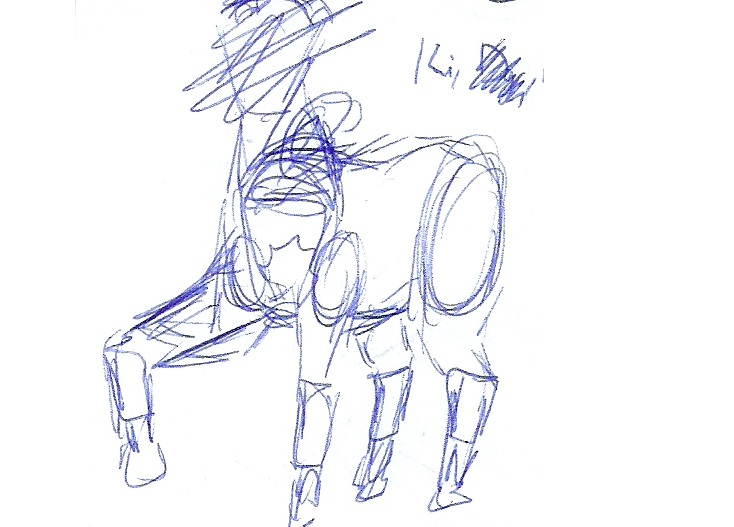
\includegraphics[width=14cm]{Images/Machines/machineHorse}
  \caption{Sketch for the Horse machine}
\end{figure}

\subsection*{Spider}
A spider-like machine that allows Sophie to climb some buildings.
\begin{figure}[H]
  \centering
  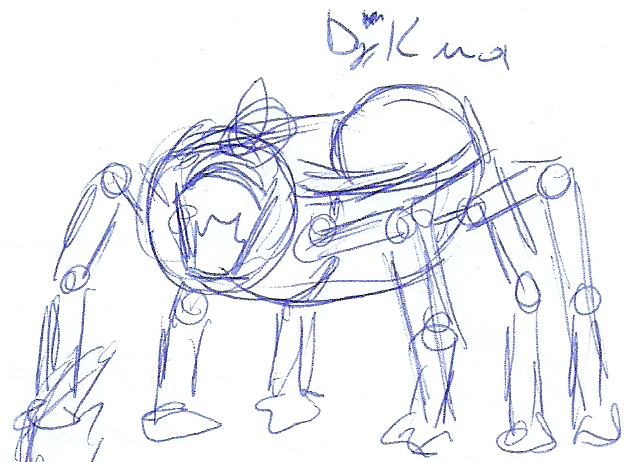
\includegraphics[width=14cm]{Images/Machines/machineSpider}
  \caption{Sketch for the Spider machine}
\end{figure}

\subsection*{Shark}
A shark-like machine that allows Sophie to sail on water.
\begin{figure}[H]
  \centering
  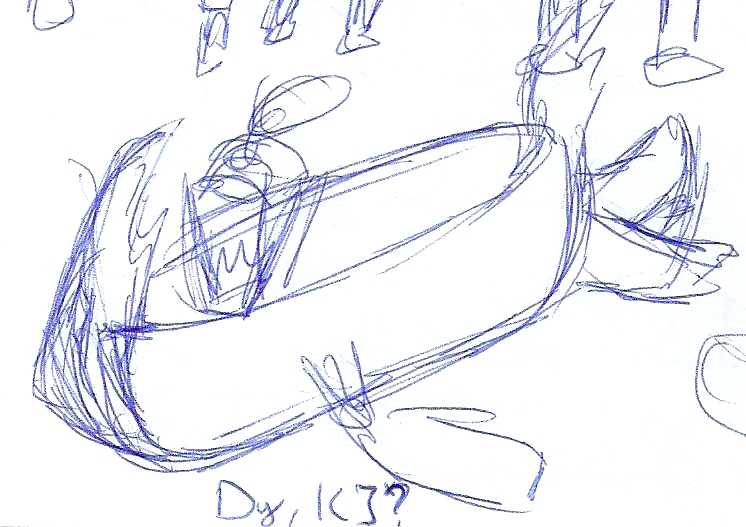
\includegraphics[width=14cm]{Images/Machines/machineShark}
  \caption{Sketch for the Shark machine}
\end{figure}

\subsection*{Wheel}
A wheel-like machine that allows Sophie to move faster on sand.
\begin{figure}[H]
  \centering
  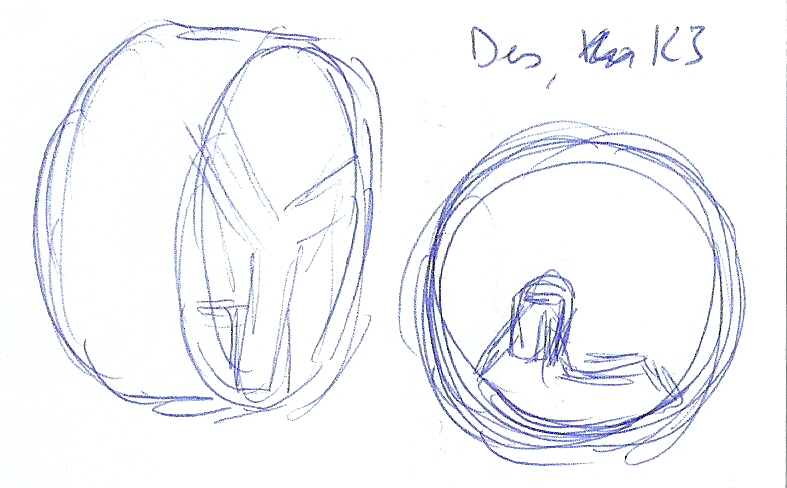
\includegraphics[width=14cm]{Images/Machines/machineWheel}
  \caption{Sketch for the Wheel machine}
\end{figure}

\subsection{Machine building puzzle}
\begin{figure}[H]
  \centering
  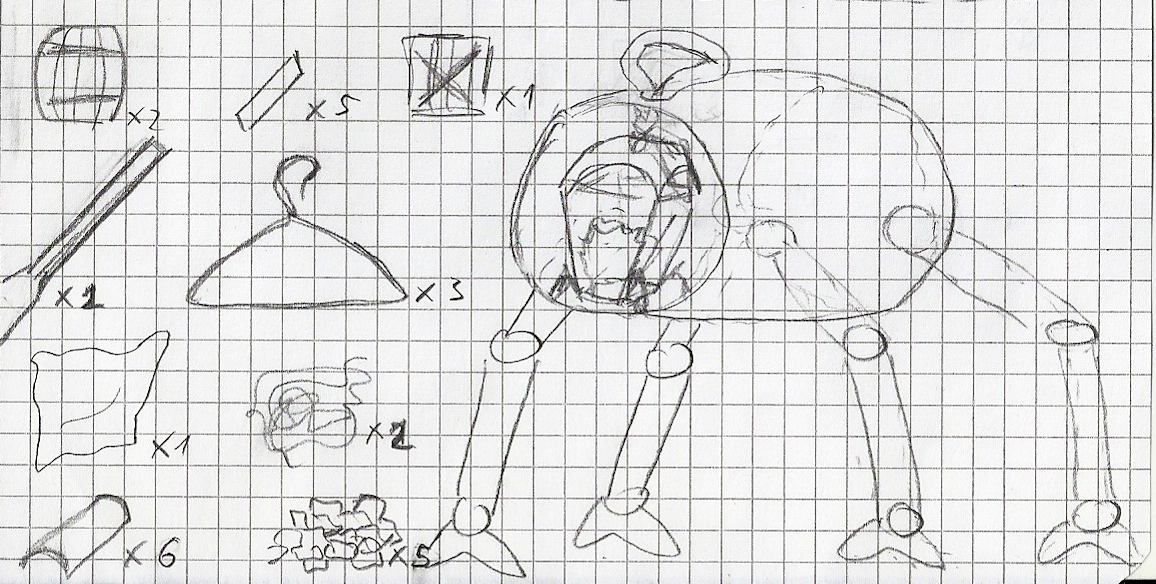
\includegraphics[width=\textwidth]{Images/Puzzles/machine}
  \caption{The Spider machine building puzzle}
\end{figure}

In order to unlock a new machine the player has to reorder the tiles of a mosaic representing the machine itself.

The tiles are randomly mixed and the player can switch any couple of tiles to reconstruct the original image.

The number of tiles is different for each puzzle to gradually increase the difficulty for the player:
\begin{itemize}
	\item \textbf{First machine}: 3 rows and 4 columns (12 tiles).
	\item \textbf{Second machine}: 3 rows and 5 columns (15 tiles).
	\item \textbf{Third machine}: 3 rows and 6 columns (18 tiles).
	\item \textbf{Last machine}: 4 rows and 6 columns (24 tiles).
\end{itemize}

\subsubsection*{Solution}
\begin{figure}[H]
  \centering
  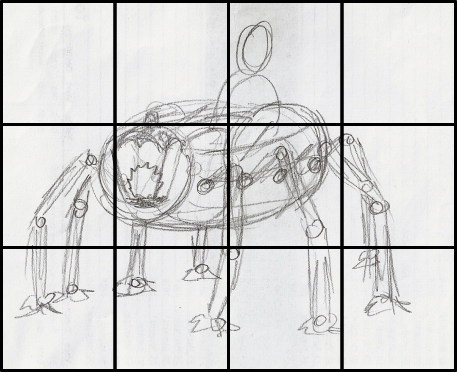
\includegraphics[width=\textwidth]{Images/Puzzles/machineSolution}
  \caption{Solution for the Spider machine building puzzle}
\end{figure}


\subsubsection*{Hints}
If the player gets stuck for some time, Sophie will tell some lines to help the player, at the same time two tiles will glitter in order to suggest to switch them.

\textbf{Sophie}: I think that piece should go there.

